
%!TEX root = ../Studienarbeit.tex

\section{Bilderkennung und -Verarbeitung}


\section{Hardwarerealisierung}

Für einen optimalen Vertreibungseffekt werden verschiedene Aktoren im System verbaut. Die einzelnen Geräte werden alle über eine externe Energieversorgung, beziehungsweise Batterie betrieben. Bei der Wahl der Batterie, ist ein wichtiges Kriterium, wie lange das System ohne Energiezufuhr funktionsfähig bleibt.
\\
Dabei wurde berücksichtigt, wie viel das System im Normalverbrauch ohne Einschalten der Aktoren verbraucht. Eine grobe Schätzung ergab, dass das System ungefähr 10 $\pm$ 2 Watt pro Stunde verbrauchen würde. Aus diesem Grund fiel die Wahl auf eine 50 Ah Autobatterie von \textit{BlackMax} \cite{Autobatterie} gefallen. Diese Batterie bietet ausreichend Kapazität, um das System über zwei Tage mit Energie zu versorgen.
\\
Ein weiterer Entscheidungsgrund für die Autobatterie ist der Strombedarf der Geräte. Wie nachfolgend beschrieben, kann die Wasserpumpe im laufenden Zustand bis zu 16 Ampere Strom beziehen. Viele leichte und kleine Batterien könnten langfristig durch diese Belastung Schaden nehmen. Da Autobatterien eine hohe Belastungsgrenze haben, sind sie für den Prototypen besser geeignet.

\subsection{Blitzlicht}

Für den Einsatz eines Abschrecklichtes mit Blitzlichtfunktion
werden zwei LED-Scheinwerfer der Marke NAIZY für 11.99€
verwendet. Die Erweiterungsleuchten sind für den Einsatz als Erweiterungsleuchten für Geländefahrzeuge gedacht. Sie sind wasserdicht und für den Außeneinsatz geeignet. Mit 1600 Lumen und grellweißem Farbton haben sie ausreichend Leistung um die Tiere abzuschrecken. Aufgrund dieser Charakteristiken und des geringen Energieverbrauchs von 18 Watt sind sie für das Abschrecksystem ausgewählt worden. \cite{am_licht}

Die zwei LED-Scheinwerfer sind an den beiden oberen Ecken der Box
befestigt. Sie werden mit Transistoren durch den Raspberry Pi gesteuert. Um einen Gewöhnungseffekt zu vermeiden sind die
Scheinwerfer mit 0.5 bis 10 Hz beschalten. Die Frequenz und Schaltung der Scheinwerfer wird in einem eigenen Thread
mittels Signalsteuerung verwirklicht.
\comment{Testen der Rust implemtierung mittels Waker?}
\comment{Bild bei Nacht aus/an + Schaltbild}

Im Schaltbild \comment{todo Schaltbild} wird die Verwendung eines
MOSFET-Treiberbausteins erkenntlich. Der Treiber ermöglicht das
schalten der Scheinwerfer. Der Treiber verfügt über eine zusätzliche GND-Leitung. Dadurch ist es möglich den Strom zu schalten, auch wenn der Signalgeber und \textit{DC-Out} nicht die selbe Masse haben.
Wenn die Transistoren mittels PWM gesteuert werden, ist diese Art der Ansteuerung notwendig. Andernfalls würde das PWM-Signal auf die falsche Masse bezogen und der Transistor nicht schalten.
\comment{todo literaturverweis}

\comment{Verkabelung, Aufbau, Herausforderungen, spezielle Lösungen}
Auswahl PI -> Liefermangel
Erstidee Multiplexer um zeitverzögerung zu reduzieren -> schlechte Kritik
% https://www.amazon.de/Arducam-Adaptermodul-Raspberry-kompatibel-Kameras/dp/B07TYL36MC/ref=sr_1_5?__mk_de_DE=%C3%85M%C3%85%C5%BD%C3%95%C3%91&crid=2KI1QVYFS8KN6&keywords=camera+adapter+raspberry&qid=1662198136&sprefix=camera+adapetr+raspberry%2Caps%2C77&sr=8-5

Zweite Idee usb-> von vornerein "komplexer" /durch zeitkacke -> irgendwie auch teuer

Dritte Idee esp32-CAM Module -> Hohe Latenzen und Zeitsynchronitätsaufwand

Viertens -> compute model + I/O shield auch teuer aber 2 csi Anschlüsse

5. Jetson mit 2 CSI Anschlüssen -> teuer und noch mehr Liefermangel

\subsection{Wasserversorgung}

integrierte Pumpe $\rightarrow$ Soll portable sein

Alternativ: Gartenschlauch mit Ventilsteuerung

\subsubsection{Pumpe}

Orientierung Gartenschlauch/Sprinkler:
Durchfluss in etwa 20L/min; Druck bis 4 Bar; Düsenspritze ca. 1-2mm Durchmesser

Pumpe: Membranpumpe $\rightarrow$ Gleichbleibende Fördermenge
bei hohen Druckunterschieden (Pumpe 1-4 Bar).
Druck Vernachlässigen und Strömungslehre mit Fördermenge
berechnen. Membranpumpe haben Druckschalter $\rightarrow$
wie ist ein/ausschaltverfahren? Delay etc. Auswahl Verwendung
von Ventil zum Durchschalten oder von Versorgungsspannung der Pumpe???
\\
Problem beim Druckventil:\\
Bei leerem Tank schaltet die Pumpe nicht ab, daher muss Schaltung über Versorgung der Pumpe durchgeführt werden.
\\
Die Pumpe arbeitet unter hoher Last. Kurzer Test bei Düsendurchmesser 1.5 mm zeigte eine Fördermenge von ca. 5 Liter pro Minute. Zudem ist durch die turbolende Strömung eine zu hohe Streuung des Wasserstrahl verursacht worden (Durchmesser 70 cm). Das Tier würde daher nur ein \enquote{tröpfeln} wahrnehmen mit geringen Störungsfaktor.

Normale Pumpe: Komplexer durch kennlinie $\rightarrow$ Berechnung des
inneren Drucks nötig und Interpolation dieser. (Meiste Pumpen
haben schon bei 1-2 Bar Probleme $\rightarrow$ Druckventil schaltet Pumpe aus.

\subsubsection{Wassertank}
Integriert oder Schlauch zu extern. Vor-/Nachteile Entscheidung?

Integriert:

Vollständig portable

;schwerer, Dichtigkeitsproblem

Extern:

Bedingt portable, einfacher zu realisieren, Systembetrachtung geringer

Wasserversorgung muss am Einsatzort möglich sein, Lange Strecken und Höhen für
Pumpe nicht gut.


\section{Dreidimensionales Zielsystem}

$\rightarrow$ Entscheidung Servo/DC?

\comment{Mit Vision Schwerpunkt der Arbeit teils/ganz in HW-Realisierung?}

\section{Kostenaufstellung}

\begin{longtable}{ p{0.15\textwidth}|p{0.2\textwidth}|p{0.5\textwidth} }
    \endfirsthead
    \multicolumn{2}{l}%
    {\textit{Fortsetzung von vorheriger Seite}} \\
    \hline
    \endhead
    \hline \multicolumn{2}{r}{\textit{Fortsetzung auf nachfolgender Seite}} \\
    \endfoot
    \endlastfoot
    \textbf{Bauteil} & \textbf{Gesamtpreis in € (inkl. Mwst.)} & \textbf{Beschreibung}\\
    \hline
    LED-Scheinwerfer
    & \centering11.99
    & Die effizienten LED-Scheinwerfer sind für die Anwendung als Erweiterungsleuchten für das Fahrzeug gedacht. \cite{am_licht} Da die LEDs den hohen Belastungen beim Einsatz am Fahrzeug standhält, werden sie den Anforderungen an einem portablem Abschrecksystem gerecht. Sie werden als Blitzlicht für das Abschrecksystem verwendet.
    \\
    Membran-pumpe
    & \centering73.35
    & Membranpumpen sind bei einfachen und kostengünstigen Anwendungen vertreten. Durch den geringen Verschleiß und einfache Wartbarkeit werden sie häufig in Frisch- und Abwasseranwendungen eingesetzt. \cite{mebranpumpe} In der Arbeit wird die Pumpe wegen ihrem geringen Verschleißes und Anschaffungskosten verwendet.
    \\
    Solarpanel
    & \centering69.99
    & Das Solarmodul wird verwendet um die Portabilität und Autarken Eigenschaften der Abschrecksystems zu gewährleisten. Solange Sonnenlicht am Einsatzort verfügbar ist, kann das Abschrecksystem mit ausreichend Energie versorgt werden um die unliebsamen Kleintiere zu erkennen.
    \\
    Autobatterie
    & \centering59.90
    & Kombiniert mit dem Solarmodul versorgt die Batterie das Abschrecksystem mit der nötigen Energie. Tagsüber wird sie mithilfe des Solarmoduls aufgeladen, während sie Nachts das System mit Energie versorgt. \cite{Autobatterie}
    \\
    Diverse Kleinteile
    & \centering{25 + X}
    & Diverse Kleinsteile werden in der Arbeit verwendet. Auch die Transistoren, die verwendet werden um die verschiedenen Aktoren an- und auszuschalten fallen unter dieser Kategorie. Aber auch die Räder, Schläuche, Kabel, Steckverbindungen und Schrauben werden hier miteinberechnet. Zusätzlich kommen die, für das Abschrecksystem angefertigten 3D-gedruckten Elemente hinzu.
    \\
    Aluminium-kiste
    & \centering{109 DM}
    & Die Aluminiumkiste ist Witterungsfest und besitzt eine gute Wärmeableitung. Alle Aktoren und Gerätschaften können in ihr vor Witterungsbedingungen geschützt untergebracht werden.
\end{longtable}

\begin{figure}
    \centering
    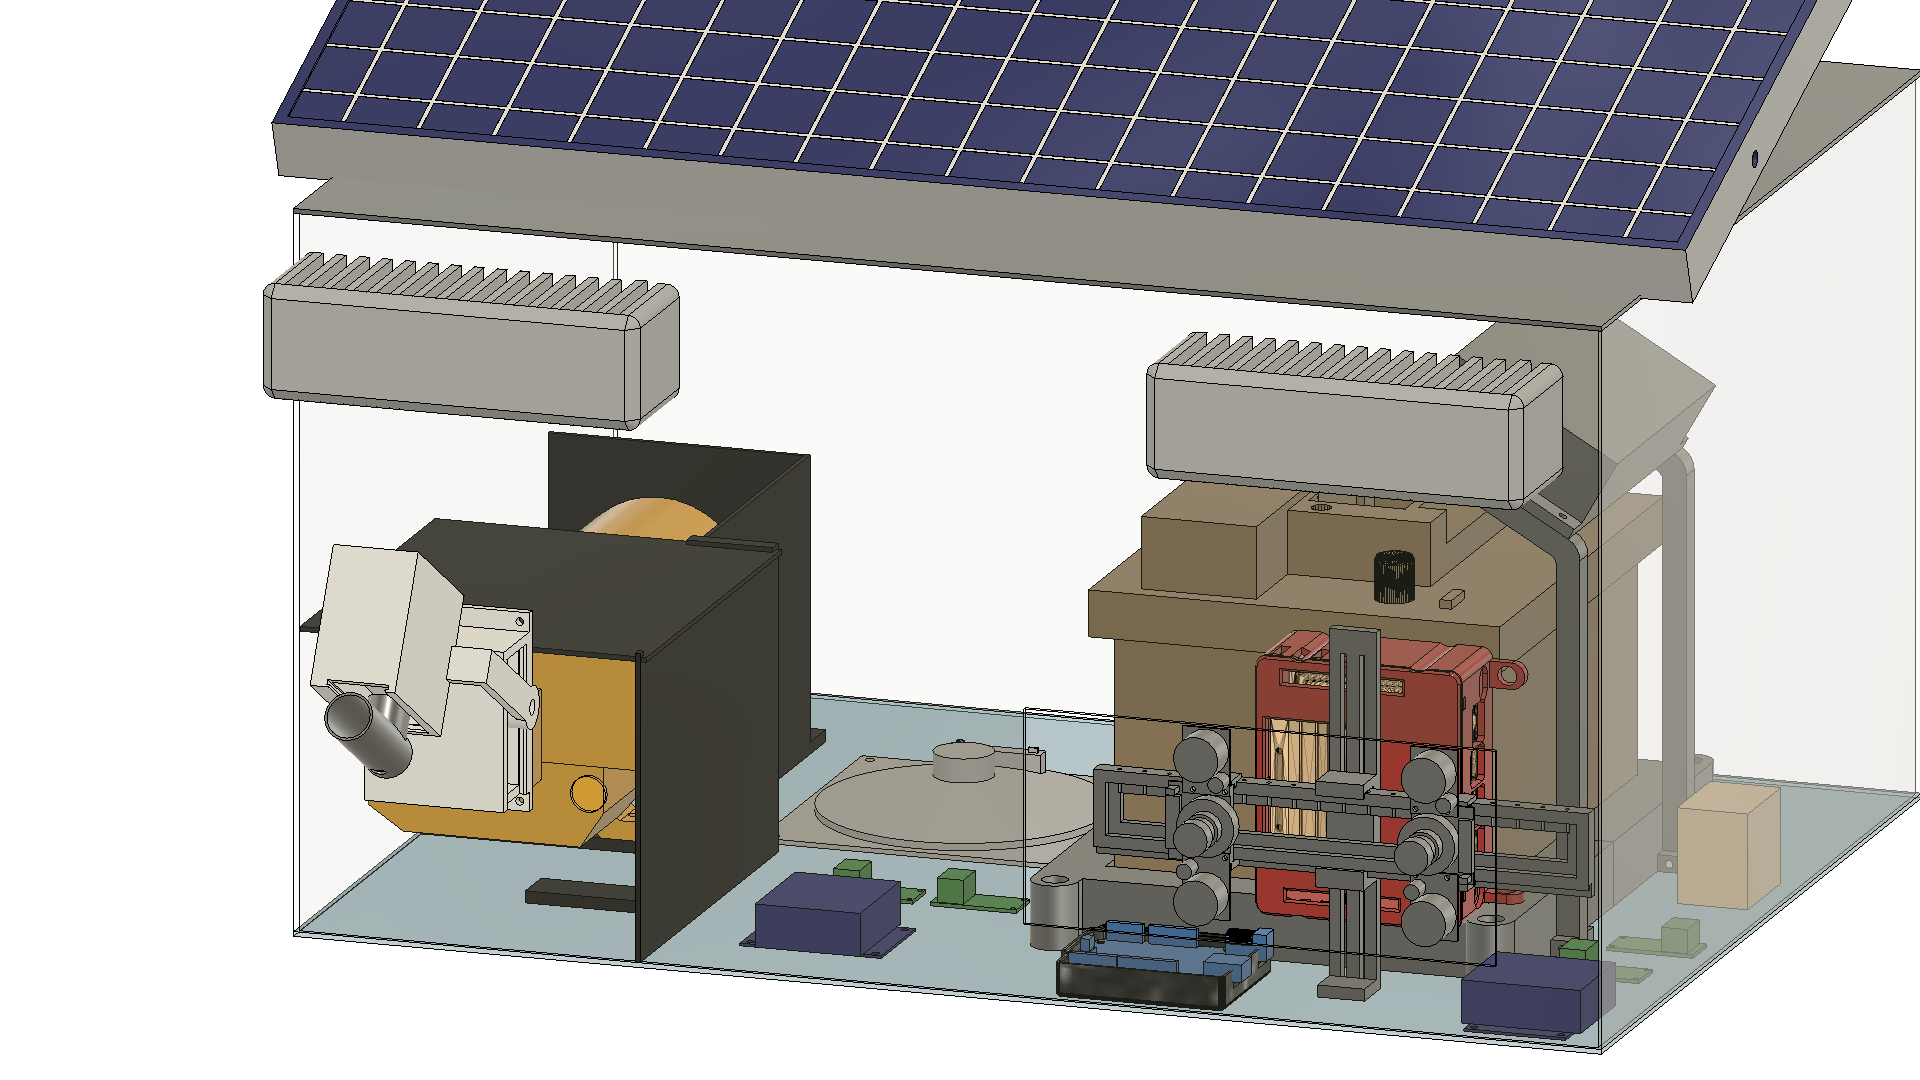
\includegraphics[width=\textwidth]{images/whole_box.png}
    \label{fig:whole_thing}
\end{figure}
